
\appendix

%%%%%%%%%%%%%%%%%%%%%%%%%%%%%%%%%%%%%%%%%%%%%%%%
% Apendice A
%%%%%%%%%%%%%%%%%%%%%%%%%%%%%%%%%%%%%%%%%%%%%%%%
\chapter{Edad escolar en diferentes Sistemas Educativos}\label{anexo:edad-educacion}

Incluso en la Unión Europea, los Sistemas Educativos difieren en la edad de escolarización de los estudiantes. Por ello, se ha confeccionado una tabla que intenta resumir la edad estándar en la que un niño está escolarizado durante las distintas etapas educativas\footnote{Se hablará de las etapas en las que el Sistema Educativo referido está bajo la responsabilidad del Ministerio de Educación (o equivalente) del propio país. Esto no excluye a la educación en centros privados.}. La información que se muestra a continuación está basado en \cite{cursos-educacion-europa} y \cite{guide-education-us}.

Se tomarán como referencia los nombres de las etapas del Sistema Educativo Español (Educación Infantil, Primaria, Secundaria y Bachillerato) para mostrar los años que pasan los estudiantes. Con respecto a la selección de países para realizar la comparación, se escogen los más representativos en los que se han realizado los estudios sobre el aprendizaje de la programación y donde más extendido están las plataformas que se mencionan en el presente documento. 


\begin{table}[!ht]
	\begin{centering}
		\begin{tabular}{c|c|c|c|c}
\emph{País} & Infantil & Primaria & Secundaria & Bachillerato\\
\hline
\emph{España} & 0-6 & 6-12 & 12-16 & 16-18\\
\emph{Estados Unidos} & 3-6 & 6-10 & 10-14 & 14-18\\
\emph{Reino Unido} & 2-5 & 5-11 & 11-16 & 16-18\\
\emph{Alemania} & 0-6 & 6-10 & 10-16 & 16-19\\
\emph{Francia} & 2-6 & 6-11 & 11-16 & 16-18\\
\emph{Bélgica} & 0-2.5/3 & 2.5/3-6 & 6-12 & 12-18\\
\emph{Irlanda} & 4-6 & 6-12 & 12-15 & 15-19\\
\end{tabular}
	\caption{Comparativa de edades de escolarización en diferentes Sistemas Educativos con respecto a las etapas del Sistema Educativo Español.}
		\label{tab:comparativa-tecnicas}
	\end{centering}
\end{table}

En el caso del Sistema Educativo Americano, existen muchas vías en la formación de un niño, como bien detalla A. Corsi-Bunker en \cite{guide-education-us}. Dependiendo de si se escoge una vía privada o dependiendo del estado, los años pueden variar. Aún así, en la figura \ref{tab:comparativa-tecnicas} se muestra el modelo estándar (sistema K-12).\footnote{Para más información sobre el Sistema Educativo Americano recomiendo que se acuda directamente a la fuente: U.S. Department of Education, National Center for Education Statistics (\url{http://nces.ed.gov})}.

\begin{figure}[!ht]
	\begin{centering}
		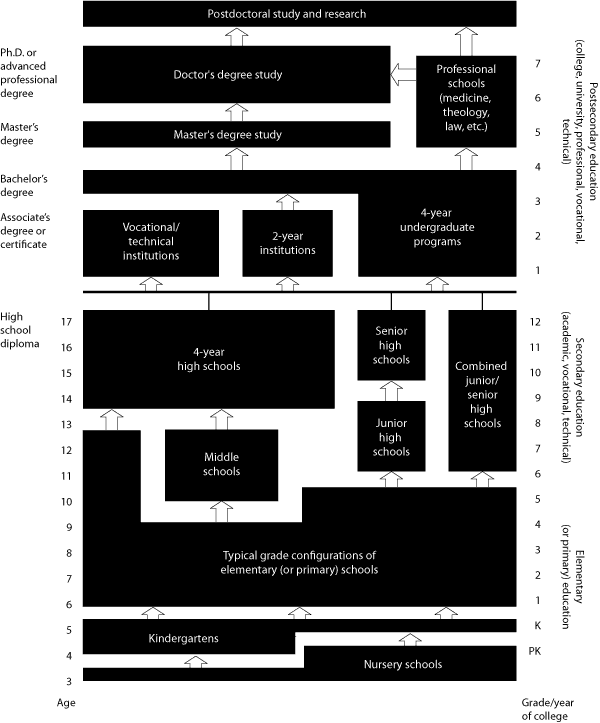
\includegraphics[width=0.75\textwidth]{images/education-usa.png}
			\caption{Tabla que muestra los típicos patrones de progresión en el Sistema Educativo Americano. Fuente: U.S. Department of Education, National Center for Education Statistics, Annual Reports Program. Obtenido de \url{http://nces.ed.gov/programs/digest/d11/figures/fig_01.asp}}
				\label{fig:education-usa}
	\end{centering}
\end{figure}





%%%%%%%%%%%%%%%%%%%%%%%%%%%%%%%%%%%%%%%%%%%%%%%%
% Apendice B
%%%%%%%%%%%%%%%%%%%%%%%%%%%%%%%%%%%%%%%%%%%%%%%%



